%!TEX root = ../thesis.tex

% \section{提案手法における従来の実験}

% \begin{itemize}
  \section{実験目的}
  簡易的なシミュレータ上で, 提案手法の有効性の検証を行う
  \section{実験装置}
  % 4.1.1で述べた簡易的なシミュレータ環境とロボットで実験を行った
  \begin{itemize}
    
    \item コンピュータとシミュレータ
    \begin{enumerate}
      \item コンピュータ\\
      OS: Ubuntu 20.04 LTS\\
      ROS: Noetic\\
      CPU: intel Core i7-10700F(4.8GHz/8コア/16スレッド)\\
      DRAM: 32GB DDR4(3200/8GB×4)
      \item nav\_cloning(学習器, 統合環境)\\
      \url{https://github.com/open-rdc/nav_cloning}
      \item waypoint\_nav(移動目標地点, 目標方向を出力)\\
      \url{https://github.com/open-rdc/waypoint_nav}
      \newpage
      \item turtlebot3 関連\\
      \url{https://github.com/open-rdc/turtlebot3}
      \item navigation(ナビゲーションパッケージ)\\
      \url{https://github.com/ros-planning/navigation}
    \end{enumerate}

    \item ロボット\\
    ロボットモデルは前報\cite{okada1}\cite{okada2}と同様, \figref{Fig:waffle_pi}に示すように, TurtleBot3 Waffle\_pi\cite{turtlebot3}へ3つのカメラを追加したモデルを用いる.

    \begin{figure}[hbtp]
      \centering
    \includegraphics[keepaspectratio, scale=0.22]
          {images/Waffle_pi.png}
    \caption{TurtleBot3 waffle\_pi with 3 cameras}
    \label{Fig:waffle_pi}
    \end{figure}

    \item 環境\\
    シミュレータ環境として, オープンソースの3DロボットシミュレータGazebo\cite{gazebo}を用いる. \figref{Fig:sim}に示すようなGazebo上で千葉工業大学津田沼キャンパス2号館3階を模した実験環境を対象に実験を行う.

    \begin{figure}[hbtp]
      \centering
    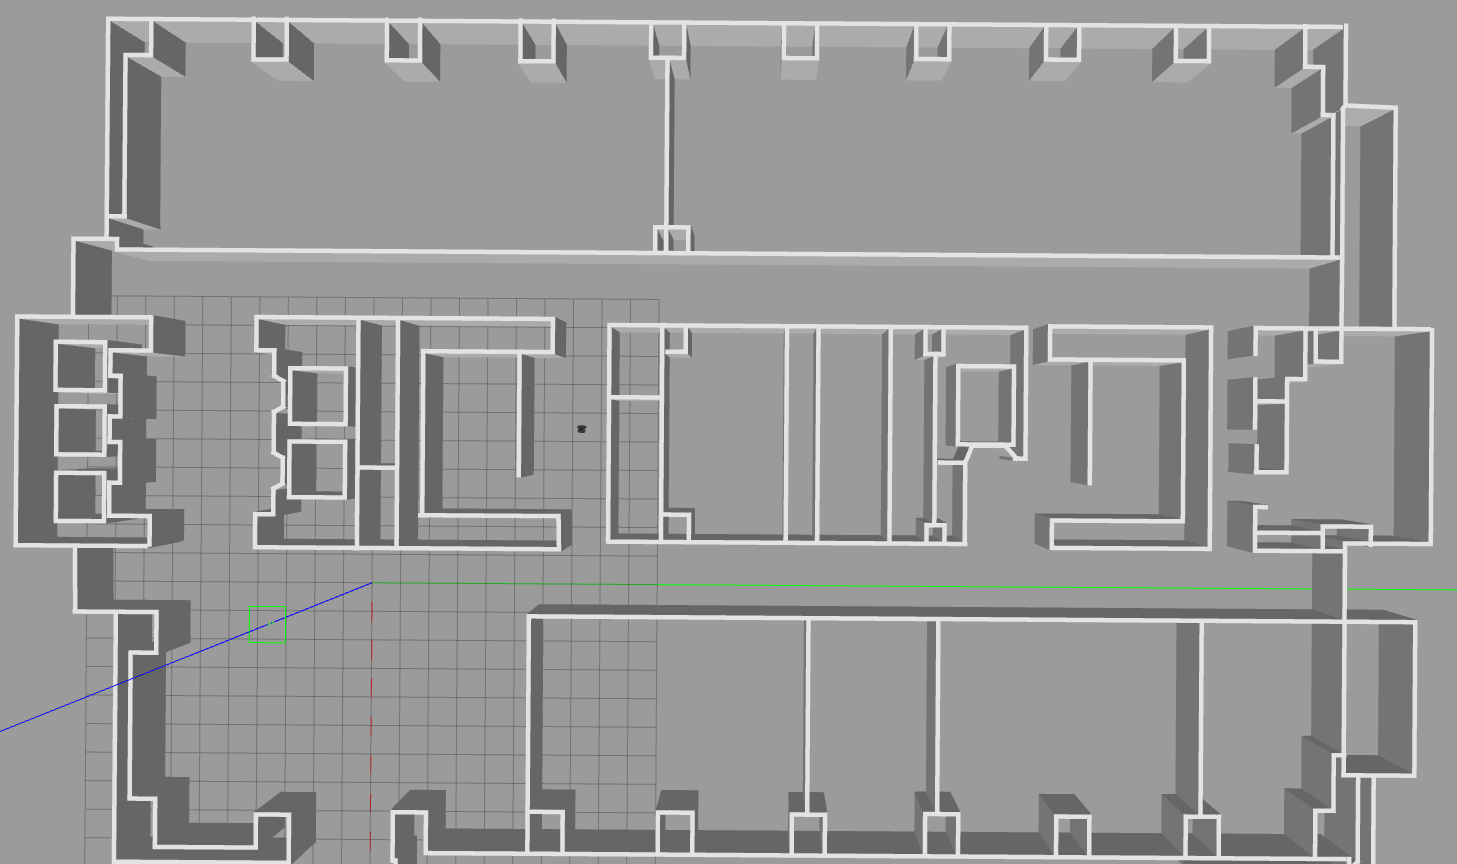
\includegraphics[keepaspectratio, scale=0.12]
          {images/tsudanuma2-3_simorg.png}
    \caption{Experimental environment of simulator}
    \label{Fig:sim}
    \end{figure}

  \end{itemize}

  \section{実験方法}
  \figref{Fig:sim_explain}のA, B地点において, \figref{Fig:select}に示すように侵入する方向が3つあり, 進むことのできる方向が2つあることから, 1箇所につき走行パターンが6つ存在する. 
また, A, B地点では, 目標方向に従って任意の経路を選択することが求められる場所である.
したがって, 実験ではA, B地点で合計12パターンの走行において, 与えた目標方向に従った行動が行えるのかを確認する.

\begin{figure}[hbtp]
  \centering
 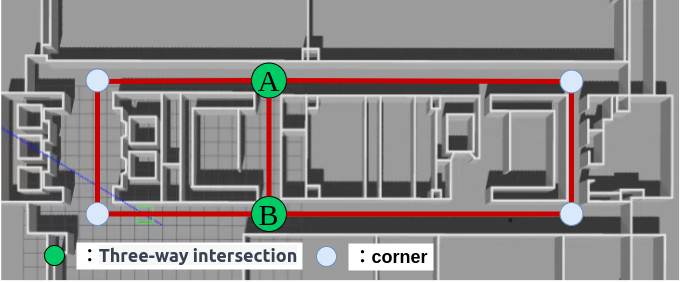
\includegraphics[keepaspectratio, scale=0.5]
      {images/sim_explain.png}
 \caption{Characteristics of passages in the experimental environment on the simulator}
 \label{Fig:sim_explain}
\end{figure}

\begin{figure}[hbtp]
  \centering
 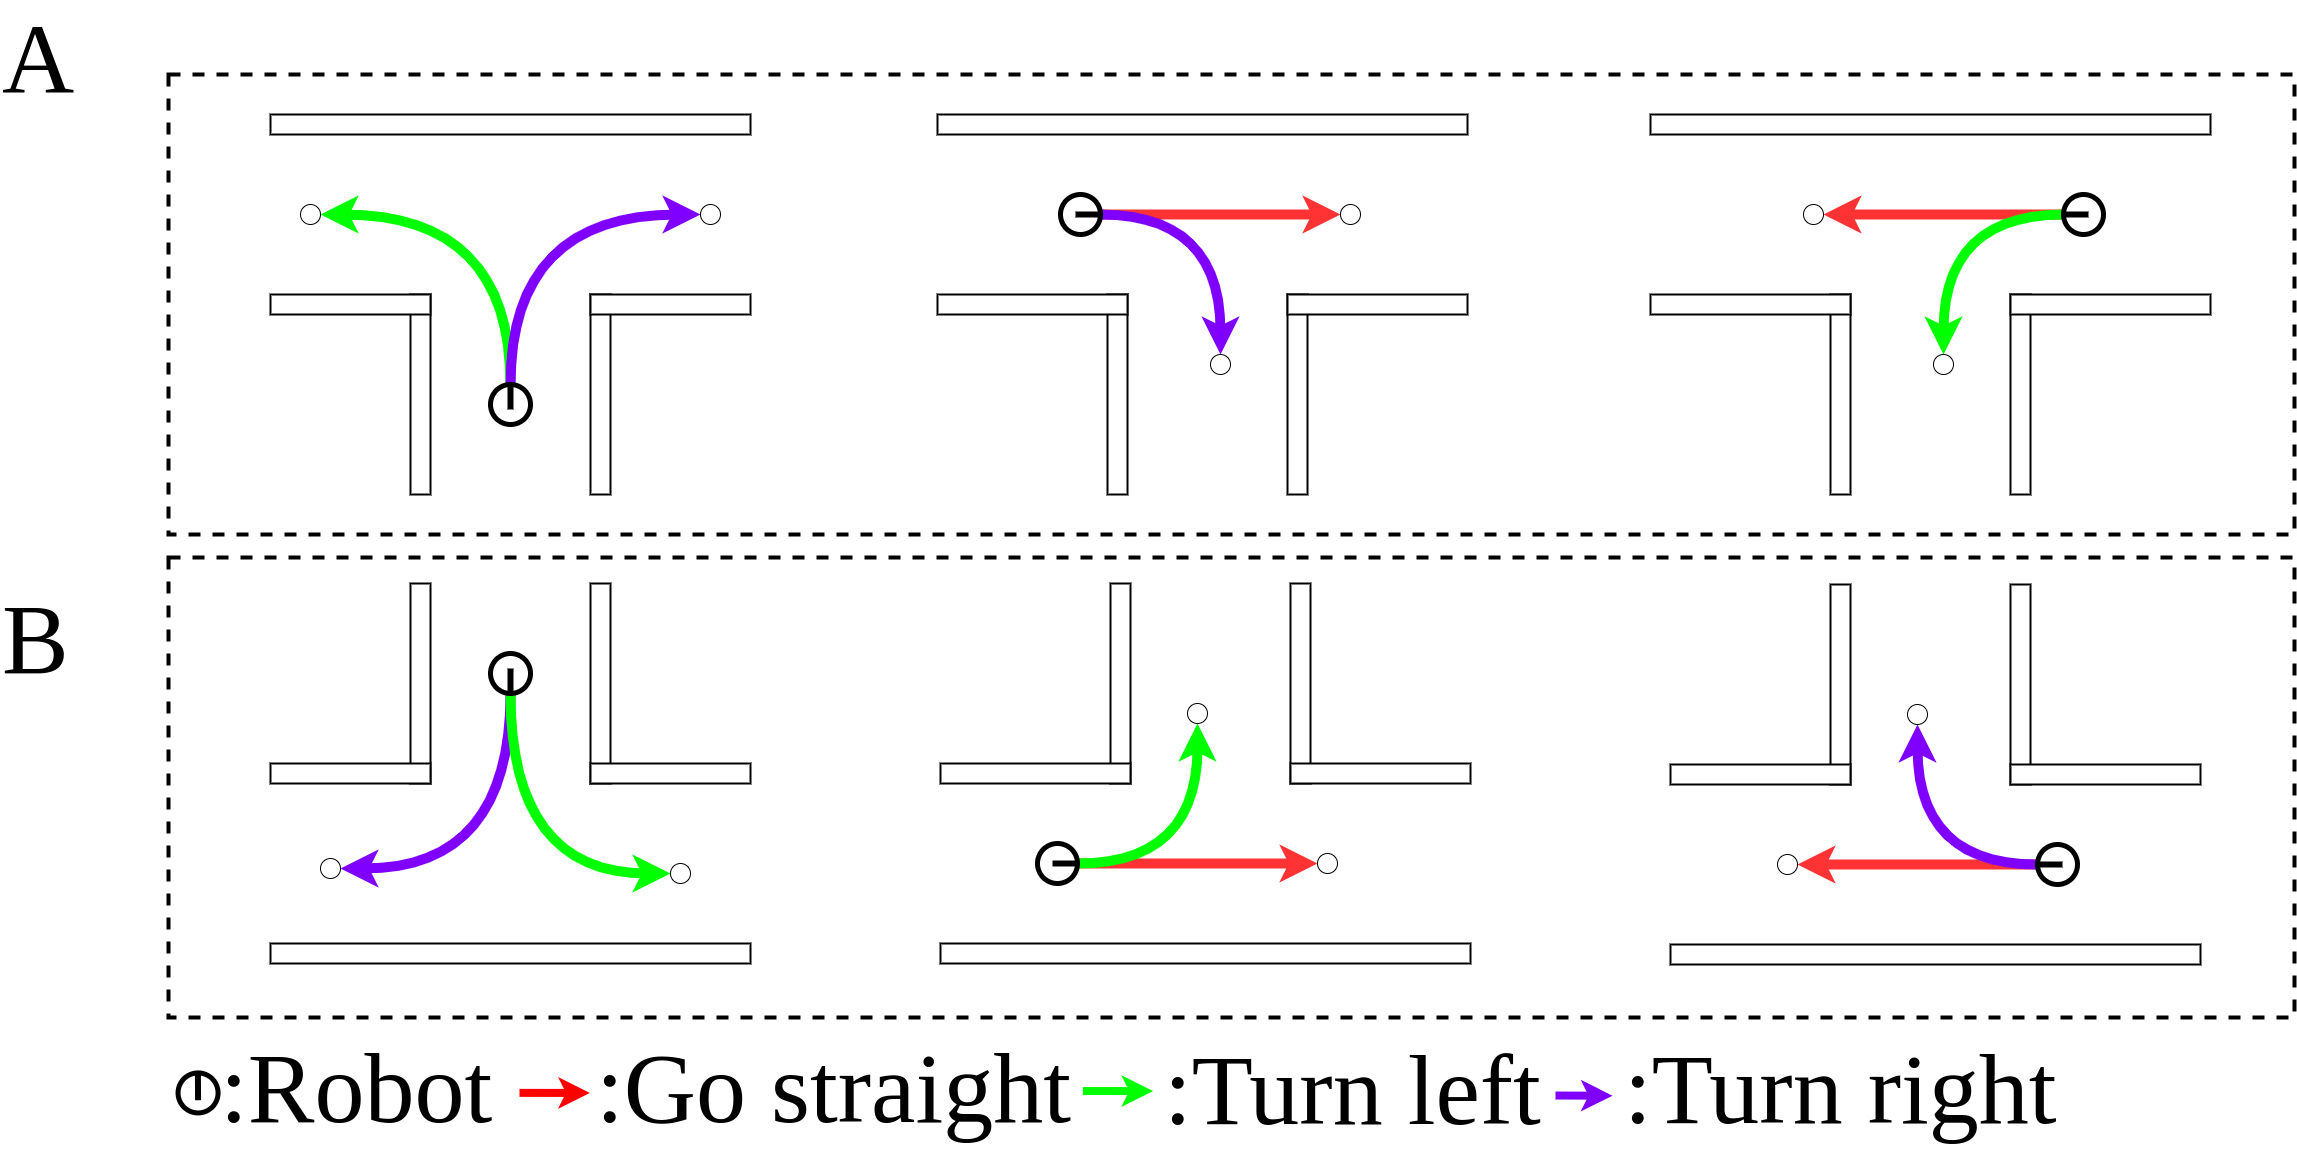
\includegraphics[keepaspectratio, scale=0.15]
      {images/select.png}
 \caption{Moving pattern at points A and B}
 \label{Fig:select}
\end{figure}

全ての走行パターンを網羅するように模倣学習を行うため, \figref{Fig:route}に示すようにaからfまでの経路を繰り返し走行させる. なお, 目標方向はwaypoint\_navから生成され, データセットに加えられる. 学習終了後, テストフェーズに移行するが, 学習時と同様にaからfまでの順番で経路をロボットに走行させる. また, テストフェーズ時にロボットが壁に衝突した場合, 経路の中央にロボットを移動させた後, 走行を再開させる.
\par
 学習を60000step実行後, テストフェーズに移行する. テストフェーズで正しい順序で経路を選択し, 走行を行えるか確認する. この一連の流れを10回繰り返し行う.

  % \newpage

  \section{実験結果}
  実験結果を\figref{Fig:60000step}に示す. この図は, それぞれの走行パターンにおいて正しく経路を選択し, 走行できた回数を表している. \tabref{table:result}に全パターンの成功回数を合計した結果を示す. なお, 分母が120であるのはテストフェーズにおいて, 全12パターンからなる経路を走行させ, 評価を行うことを10回繰り返したためである. 
  \par
  \tabref{table:result}に示すように, 目標方向に従って113/120回, 正しい経路を選択する様子が見られた. 

\vspace{1cm}

\begin{figure}[hbtp]
  \centering
 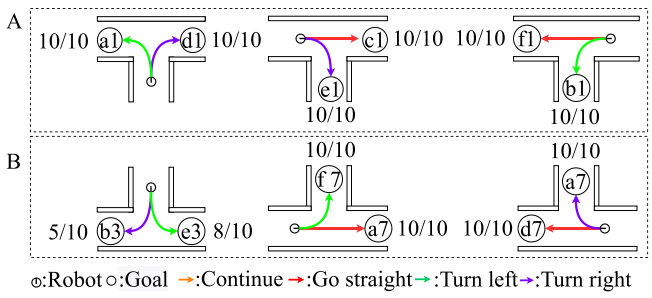
\includegraphics[keepaspectratio, scale=0.5]
      {images/60000step.png}
 \caption{Experimental results for each moving pattern from \cite{mech}}
 \label{Fig:60000step}
\end{figure}

\vspace{1cm}

\begin{table}[hbtp]
  \caption{Experimental results}
  \label{table:result}
  \centering
  \begin{tabular}{|c|c|c|}
    \hline
    Experiments & Step & Total result\\
    \hline
    Conventional & 60000 & 113/120(94.2\%)\\
    \hline
  \end{tabular}
\end{table}

% \end{itemize}

\newpage